\documentclass[mathserif,serif,unicode]{beamer}
\usepackage[utf8]{inputenc}
\usepackage[russian]{babel}
\usepackage{amssymb,amsmath,mathrsfs,graphicx}
\usepackage{array}
\usepackage{ulem}\normalem
\usepackage{tabularx,multirow}
\usepackage{booktabs}
\usepackage{subcaption}
\usepackage[linesnumbered,vlined]{algorithm2e}

%\newrobustcmd*{\footlessfullcite}{\AtNextCite{\renewbibmacro{booktitle}{}\renewbibmacro{pages}{}\renewbibmacro{in:}{}}\footfullcite}
%\bibliography{references}

\setbeamercolor{footline}{fg=black}
\setbeamerfont{footline}{series=\bfseries}
\setbeamertemplate{navigation symbols}{}

% Beamer themes and colors
\usetheme{Frankfurt}
\usecolortheme{seahorse}
\usefonttheme[onlylarge]{structurebold}
\setbeamerfont*{frametitle}{size=\normalsize,series=\bfseries}

\hypersetup{
  colorlinks=true,
  linkcolor=black,
  urlcolor=blue
  }

\newcommand{\Tr}{\mathsf{\scriptstyle T}}
\DeclareMathOperator*{\argmin}{arg\,min}
\DeclareMathOperator*{\argmax}{arg\,max}
%\newcommand{\Prob}{\mathsf{P}}
\newcommand{\Expect}{\mathsf{E}}
\newcommand{\const}{\mathsf{const}}
%\newcommand{\arg}{\mathsf{arg}}
\newcommand{\aggr}{\mathsf{aggr}}
\newcommand{\diag}{\mathsf{diag}}
\newcommand{\corr}{\mathsf{corr}}
\newcommand{\cov}{\mathsf{cov}}
\newcommand{\Sim}{\mathsf{sim}}
\newcommand{\Dir}{\mathsf{Dir}}
\newcommand{\KL}{\mathsf{KL}}
\newcommand{\tsum}{\mathop{\textstyle\sum}\limits}
\newcommand{\tprod}{\mathop{\textstyle\prod}\limits}
\renewcommand{\epsilon}{\varepsilon}
\newcommand{\eps}{\epsilon}
\renewcommand{\geq}{\geqslant}
\renewcommand{\leq}{\leqslant}
\renewcommand{\ge}{\geqslant}
\renewcommand{\le}{\leqslant}
\newcommand{\T}{\textsf{\upshape т}}
\def\XX{\mathbb{X}}
\def\YY{\mathbb{Y}}
\def\RR{\mathbb{R}}
\def\LL{{\mathscr L}}
\def\cL{\mathscr{L}}

\title{1000 и 1 боль при конвертации модели}
\author{Андрей~Шадриков\\
%  Сбербанк
}
\date{Октябрь~2020}

\usepackage{graphicx,natbib}

\begin{document}

\begin{frame}[plain]
  \titlepage
\end{frame}

%%%%%%%%%%%%%%%%%%%%%%%%%%%%%%%%%%%%%%%%%%%%%%%%%%%%%%%%%%%%%%%%%%%%%%%%
\section{Введение}

\begin{frame}{Зачем конвертировать?}

\begin{itemize}
    \item Фреймворки в исследовании:\\
    \begin{figure}[h]
        \centering
        
\includegraphics[width=0.9\textwidth]{images/high-level.png}
    \end{figure}
\vspace{5mm}
    \item Фреймворки в продакшене:\\
    \begin{figure}
        \centering
        
\includegraphics[width=0.9\textwidth]{images/low-level.png}
    \end{figure}
\end{itemize}

\end{frame}

%%%%%%%%%%%%%%%%%%%%%%%%%%%%%%%%%%%%%%%%%%%%%%%%%%%%%%%%%%%%%%%%%%%%%%%%
\section{Проблемы}

\begin{frame}{Откуда возникают проблемы?}

\begin{itemize}
    \item Не полная поддержка слоёв.
    \item Разный формат слоёв (NonMaximumSuppression, Upsample).
    \item Конвертаторы не поддерживают последние версии фреймворков.
    \item Не всегда можно оценить скорость работы модели в проде.
    \item Некорректная сериализация моделей.
\end{itemize}
    
\end{frame}

\begin{frame}{Есть же туториалы!}
    \begin{itemize}
        \item У каждого фреймворка есть свои способы конвертировать модели.
        \item Часто рассматриваются только базовые случаи.
        \item Могут требовать старых версий фреймворков для стабильной работы.
    \end{itemize}

\end{frame}

%%%%%%%%%%%%%%%%%%%%%%%%%%%%%%%%%%%%%%%%%%%%%%%%%%%%%%%%%%%%%%%%%%%%%%%%
\section{ONNX}

\begin{frame}{Open Neural Network Exchange}
    
    \begin{figure}
        
\includegraphics[width=0.5\textwidth]{images/ONNX_logo_main.png}
    \end{figure}

    \begin{itemize}
        \item Инициатива от Facebook и Microsoft для конвертации между PyTorch, Caffe2, CNTK.
        \item Позже поддержали другие команды.
        \vspace{5mm}
        \item Статический граф через protobuf.
        \item Версионность используемых операторов.
    \end{itemize}
\end{frame}

\begin{frame}{Что хорошо?}
    \begin{itemize}
        \item Большая поддержка конвертации между фреймворками.
        \item Большое коммьюнити, поддерживающее редкие конвертаторы.
        \item Активное развитие.
        \item Версии opset'ов для хранения старых моделей.
    \end{itemize}
\end{frame}

\begin{frame}{Когда не надо использовать}

\begin{itemize}
    \item Разработка и прод в одной экосистеме (TensorFlow, MxNet).
    \item Конвертация через ONNX требует больше усилий, чем конвертация напрямую.
    \item Модель оптимизировалась под конкретный фреймворк (и это не ONNX).
\end{itemize}
    
\end{frame}

\begin{frame}{Что хотелось бы}

\begin{itemize}
    \item Отладка моделей (вывод типов, размерностей).
    \item Мета-поля для слоёв.
    \item Более удобные инструменты работы с сериализованными моделями.
\end{itemize}
    
\end{frame}

\begin{frame}{XKCD \#927}
    \begin{figure}
        \centering
        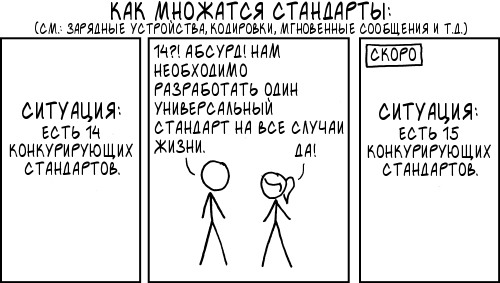
\includegraphics[width=0.8\textwidth]{images/927_v4.png}
    \end{figure}
\end{frame}

\begin{frame}{Альтернативы}

    TensorFlow
    \begin{itemize}
        \item Очень популярный, большая поддержка.
        \item Можно не выходить за рамки экосистемы.
        \item Мало конвертаций.
    \end{itemize}
\vspace{5mm}
    MMdnn
    \begin{itemize}
        \item Старее ONNX.
        \item Поддерживается очень малым числом участников.
        \item Собственный внутренний формат не стандартизован.
    \end{itemize}
\end{frame}

%%%%%%%%%%%%%%%%%%%%%%%%%%%%%%%%%%%%%%%%%%%%%%%%%%%%%%%%%%%%%%%%%%%%%%%%
\section{Примеры}

\subsection{PyTorch в ONNX}

\begin{frame}{PyTorch в ONNX}

\begin{block}{}
    \begin{figure}
        \centering
        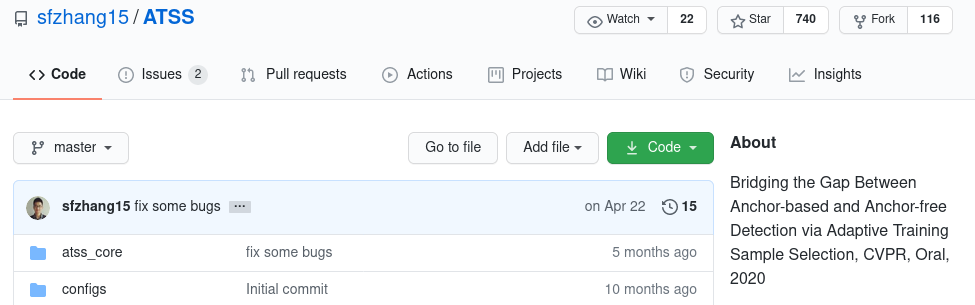
\includegraphics[width=\textwidth]{images/atss.png}
    \end{figure}
\end{block}
    
\end{frame}

\begin{frame}{Не всё так просто}
\begin{block}{}
\begin{figure}
    \centering
    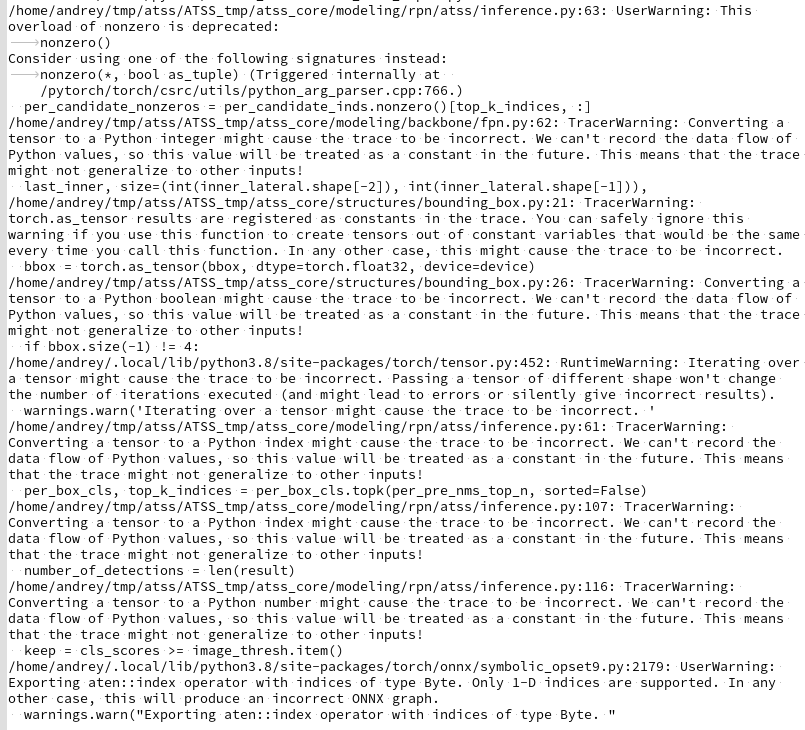
\includegraphics[width=\textwidth]{images/conv_warn.png}
\end{figure}
\end{block}
\end{frame}

\begin{frame}{Не всё так просто}
\begin{alertblock}{}
\begin{figure}
    \centering
    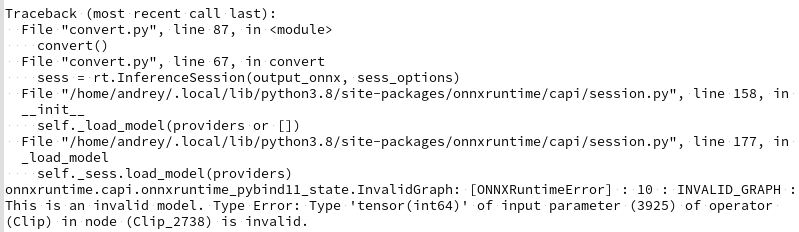
\includegraphics[width=\textwidth]{images/conv_error.png}
\end{figure}
\end{alertblock}
\end{frame}

\begin{frame}{Особенности конвертации из PyTorch}
PyTorch при конвертации использует собственное внутреннее представление через trace:
    \begin{itemize}
        \item Операции должны выполняться над объектами torch.Tensor.
        \item In-place операции скорее всего создадут неверный граф (о чём предупреждает конвертатор).
        \item Control flow посчитается один раз.
        \item Проверять корректность модели лучше на других данных, что использовались при конвертации.
    \end{itemize}
\end{frame}

\subsection{MxNet в TensorFlow}

\begin{frame}{MxNet в TensorFlow}

\begin{block}{}
    \begin{figure}
        \centering
        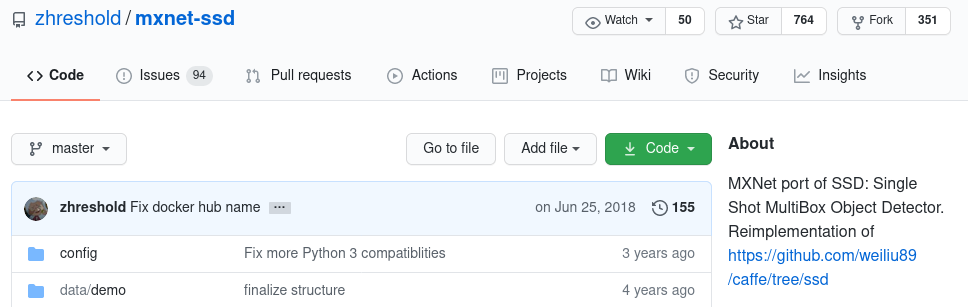
\includegraphics[width=\textwidth]{images/mxnet_ssd.png}
    \end{figure}
\end{block}
    
\end{frame}

\begin{frame}{Конвертатор из MxNet поддерживает мало}

\begin{block}{Официальная документация}
    \begin{figure}
        \centering
        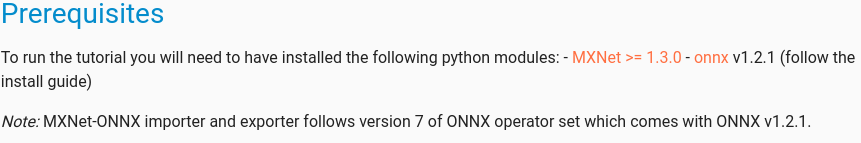
\includegraphics[width=\textwidth]{images/mxnet_onnx.png}
    \end{figure}
\end{block}
\vspace{5mm}
В последней стабильной версии ONNX v1.7.0 версия операторов 12-я, и не все имеют forward-совместимость.
    
\end{frame}

\begin{frame}{Можно обойтись тем, что есть}

\begin{itemize}
    \item<1-> Нам нужна на самом деле 10-я версия операторов.
    \item<1-> Почти все операторы имеют forward-совместимость.
    \item<1-> Слой для якорей и декодинга нужно переписать.
    \item<1-> Остаётся дело за малым --- нужно выкрутиться с NonMaximumSuppression.
    \item<2-> Сконвертируем модель без него, а затем добавим в граф TensorFlow.
\end{itemize}
    
\end{frame}

%%%%%%%%%%%%%%%%%%%%%%%%%%%%%%%%%%%%%%%%%%%%%%%%%%%%%%%%%%%%%%%%%%%%%%%%
\section{Заключение}

\begin{frame}{Что хотелось показать?}

\begin{itemize}
    \item Задача конвертации возникает достаточно часто.
    \item Неожиданные моменты могут потребовать много работы.
    \item Обсуждайте итоговые особенности продакшена заранее.
    \item ONNX хорошо использовать для сериализации моделей.
    \item Иногда проще менять граф в нужном фреймворке.
\end{itemize}
    
\end{frame}

\begin{frame}{Что за рамками}

\begin{itemize}
    \item Редкие специфичные модели (Grid Sample).
    \item Рекурентные модели.
    \item Не нейронки.
    \item Отладка и проверка корректности моделей.
    \item Мобильные и другие платформо-специфичные фреймворки.
\end{itemize}
    
\end{frame}

\begin{frame}[plain]

\centering \Huge
Спасибо за внимание!

\vspace{17mm}
\Large
\begin{tabularx}{50mm}{Xl}
      \noindent\parbox[c]{\hsize}{
          
\includegraphics[width=7mm]{images/ods.png}
      }
      & @vuvko \\
      \noindent\parbox[c]{\hsize}{
          
\includegraphics[width=7mm]{images/1200px-Telegram_2019_Logo.png}
      }
      & @vuvko \\
      \noindent\parbox[c]{\hsize}{
          
\includegraphics[width=7mm]{images/GitHub-Mark-120px-plus.png}
      }
      & vuvko \\
      \noindent\parbox[c]{\hsize}{
          
\includegraphics[width=7mm]{images/1920px-XMPP_logo.svg.png}
      }
      & vuvko@fmap.me \\
      \noindent\parbox[c]{\hsize}{
          
\includegraphics[width=7mm]{images/1200px-Gmail_Icon.svg.png}
      }
      & vuvko@fmap.me
\end{tabularx}
    
\end{frame}

\end{document}
